\documentclass[12pt,letterpaper]{report}
\usepackage[utf8]{inputenc}
\usepackage{amsmath}
\usepackage{amsfonts}
\usepackage{amssymb}
\usepackage{pdfpages}
\usepackage{graphicx}
\graphicspath{{../sharedfiles/}}
\usepackage[left=0.50in, right=0.50in, top=0.50in, bottom=0.50in]{geometry}
\author{Anthony Odenthal}
\author{National Conference of Volunteer Examiners; edited by Anthony Odenthal KE7OSN}
\title{Amateur Radio General Class Exam Questions and Answers for July 2011 to July 2015}
\begin{document}
\maketitle
\section{Preamble}
The following is the entire question pool for the General class amateur radio exam with answers. The text comes from the NCVEC National Conference of Volunteer Examiners website http://www.ncvec.org/page.php?id=358 on November 21 2013 and edited to remove the distractors (wrong answers). For questions with the answer "All of the above" the distractors were left in place for the information of anyone using this document. This document also lacks the list of corrections and modifications the original had.

Each subelement indicates the number of groups and the number of exam questions that comes form that subelement. Questions are formatted as Question Number (Letter of the correct Answer) [FCC rule number if applicable] question, the letter and answer for the correct response is listed on the second line.
\tableofcontents

\chapter*{Syllabus}
General Class Question Pool Syllabus 2011-2015 


SUBELEMENT G1 - COMMISSION'S RULES [5 Exam Questions - 5 Groups]

G1A - General Class control operator frequency privileges; primary and secondary allocations

G1B - Antenna structure limitations; good engineering and good amateur practice; beacon operation; restricted operation; retransmitting radio signals

G1C - Transmitter power regulations; data emission standards

G1D - Volunteer Examiners and Volunteer Examiner Coordinators; temporary identification

G1E - Control categories; repeater regulations; harmful interference; third party rules; ITU regions

SUBELEMENT G2 - OPERATING PROCEDURES [5 Exam Questions - 5 Groups]

G2A Phone operating procedures; USB/LSB utilization conventions; procedural signals; breaking into a QSO in progress; VOX operation

G2B - Operating courtesy; band plans, emergencies, including drills and emergency communications

G2C - CW operating procedures and procedural signals, Q signals and common abbreviations; full break in

G2D - Amateur Auxiliary; minimizing interference; HF operations

G2E - Digital operating: procedures, procedural signals and common abbreviations

SUBELEMENT G3 - RADIO WAVE PROPAGATION [3 Exam Questions - 3 Groups]

G3A - Sunspots and solar radiation; ionospheric disturbances; propagation forecasting and indices

G3B - Maximum Usable Frequency; Lowest Usable Frequency; propagation

G3C - Ionospheric layers; critical angle and frequency; HF scatter; Near Vertical Incidence Sky waves

SUBELEMENT G4 - AMATEUR RADIO PRACTICES [5 Exam Questions - 5 groups]

G4A - Station Operation and setup

G4B - Test and monitoring equipment; two-tone test

G4C - Interference with consumer electronics; grounding; DSP

G4D - Speech processors; S meters; sideband operation near band edges

G4E - HF mobile radio installations; emergency and battery powered operation

SUBELEMENT G5 - ELECTRICAL PRINCIPLES [3 exam questions - 3 groups]

G5A - Reactance; inductance; capacitance; impedance; impedance matching

G5B - The Decibel; current and voltage dividers; electrical power calculations; sine wave root-mean-square (RMS) values; PEP calculations

G5C - Resistors, capacitors and inductors in series and parallel; transformers

SUBELEMENT G6 - CIRCUIT COMPONENTS [3 exam question - 3 groups]

G6A - Resistors; capacitors; inductors

G6B - Rectifiers; solid state diodes and transistors; vacuum tubes; batteries

G6C - Analog and digital integrated circuits (IC's); microprocessors; memory; I/O devices; microwave IC's (MMIC's ); display devices

SUBELEMENT G7 - PRACTICAL CIRCUITS [3 exam question - 3 groups]

G7A - Power supplies; schematic symbols

G7B - Digital circuits; amplifiers and oscillators

G7C - Receivers and transmitters; filters, oscillators

SUBELEMENT G8 - SIGNALS AND EMISSIONS [2 exam questions  - 2 groups]

G8A - Carriers and modulation: AM; FM; single and double sideband; modulation envelope; overmodulation

G8B - Frequency mixing; multiplication; HF data communications; bandwidths of various modes; deviation

SUBELEMENT G9 - ANTENNAS AND FEED LINES [4 exam questions - 4 groups]

G9A - Antenna feed lines: characteristic impedance and attenuation; SWR calculation, measurement and effects; matching networks

G9B - Basic antennas

G9C - Directional antennas

G9D - Specialized antennas

SUBELEMENT G0 - ELECTRICAL AND RF SAFETY [2 exam Questions - 2 groups]

G0A - RF safety principles, rules and guidelines; routine station evaluation

G0B - Safety in the ham shack: electrical shock and treatment, safety grounding, fusing, interlocks, wiring, antenna and tower safety

General Class Question Pool Effective July 1, 2011 - June 30, 2015
\chapter{Subelement G1 - Commission's Rules: 5 Questions}
\section{G1A - General Class control operator frequency privileges; primary and secondary allocations}

G1A01 (C) [97.301(d), 97.303(s)] On which of the following bands is a General Class license holder granted all amateur frequency privileges?\\
C. 160, 60, 30, 17, 12, and 10 meters\\

G1A02 (B) [97.305] On which of the following bands is phone operation prohibited?\\
B. 30 meters\\

G1A03 (B) [97.305] On which of the following bands is image transmission prohibited? \\
B. 30 meters\\

G1A04 (D) [97.303 (s)] Which of the following amateur bands is restricted to communication on only specific channels, rather than frequency ranges?\\
D. 60 meters\\

G1A05 (A) [97.301(d)] Which of the following frequencies is in the General Class portion of the 40 meter band?\\
A. 7.250 MHz\\

G1A06 (D) [97.301(d) Which of the following frequencies is in the 12 meter band?\\
D. 24.940 MHz\\

G1A07 (C) [97.301(d)] Which of the following frequencies is within the General Class portion of the 75 meter phone band?\\
C. 3900 kHz\\

G1A08 (C) [97.301(d)] Which of the following frequencies is within the General Class portion of the 20 meter phone band?\\
C. 14305 kHz\\

G1A09 (C) [97.301(d)]  Which of the following frequencies is within the General Class portion of the 80 meter band?\\
C. 3560 kHz\\

G1A10 (C) [97.301(d)] Which of the following frequencies is within the General Class portion of the 15 meter band?\\
C. 21300 kHz\\

G1A11 (D) [97.301(d)]  Which of the following frequencies is available to a control operator holding a General Class license?\\
A. 28.020 MHz\\
B. 28.350 MHz\\
C. 28.550 MHz\\
D. All of these choices are correct\\

G1A12 (B) [97.301] When General Class licensees are not permitted to use the entire voice portion of a particular band, which portion of the voice segment is generally available to them? \\
B. The upper frequency end\\

G1A13 (D) [97.303] Which, if any, amateur band is shared with the Citizens Radio Service?\\
D. None\\

G1A14 (C) [97.303] Which of the following applies when the FCC rules designate the Amateur Service as a secondary user on a band?\\
C. Amateur stations are allowed to use the band only if they do not cause harmful interference to primary\\ users

G1A15 (D) [97.303] What is the appropriate action if, when operating on either the 30 or 60 meter bands, a station in the primary service interferes with your contact? \\
D. Move to a clear frequency\\

\section{G1B - Antenna structure limitations; good engineering and good amateur practice; beacon operation; restricted operation; retransmitting radio signals}

G1B01 (C) [97.15(a)] What is the maximum height above ground to which an antenna structure may be erected without requiring notification to the FAA and registration with the FCC, provided it is not at or near a public use airport?\\
C. 200 feet\\

G1B02 (D) [97.203(b)] With which of the following conditions must beacon stations comply?\\
D. There must be no more than one beacon signal in the same band from a single location\\

G1B03 (A) [97.3(a)(9)] Which of the following is a purpose of a beacon station as identified in the FCC Rules?\\
A. Observation of propagation and reception\\

G1B04 (A) [97.113(b)] Which of the following must be true before amateur stations may provide communications to broadcasters for dissemination to the public?\\
A. The communications must directly relate to the immediate safety of human life or protection of property and there must be no other means of communication reasonably available before or at the time of the event\\

G1B05 (D) [97.113(a)(5),(e)] When may music be transmitted by an amateur station?\\
D. When it is an incidental part of a manned space craft retransmission\\

G1B06 (B) [97.113(a)(4) and 97.207(f)] When is an amateur station permitted to transmit secret codes?\\
B. To control a space station\\

G1B07 (B) [97.113(a)(4)] What are the restrictions on the use of abbreviations or procedural signals in the Amateur Service?\\
B. They may be used if they do not obscure the meaning of a message\\

G1B08 (D) When choosing a transmitting frequency, what should you do to comply with good amateur practice?\\
A. Review FCC Part 97 Rules regarding permitted frequencies and emissions.\\
B. Follow generally accepted band plans agreed to by the Amateur Radio community.\\
C. Before transmitting, listen to avoid interfering with ongoing communication\\
D. All of these choices are correct\\

G1B09 (A) [97.113(a)(3)] When may an amateur station transmit communications in which the licensee or control operator has a pecuniary (monetary) interest?\\
A. When other amateurs are being notified of the sale of apparatus normally used in an amateur station and such activity is not done on a regular basis\\

G1B10 (C) [97.203(c)] What is the power limit for beacon stations?\\
C. 100 watts PEP output\\

G1B11 (C) [97.101(a)] How does the FCC require an amateur station to be operated in all respects not specifically covered by the Part 97 rules?\\
C. In conformance with good engineering and good amateur practice\\

G1B12 (A) [97.101(a)] Who or what determines "good engineering and good amateur practice" as applied to the operation of an amateur station in all respects not covered by the Part 97 rules?\\
A. The FCC\\

\section{G1C - Transmitter power regulations; data emission standards}


G1C01 (A) [97.313(c)(1)] What is the maximum transmitting power an amateur station may use on 10.140 MHz?\\
A. 200 watts PEP output\\

G1C02 (C) [97.313(a),(b)]  What is the maximum transmitting power an amateur station may use on the 12 meter band?\\
C. 1500 watts PEP output\\

G1C03 (A) [97.303s]  What is the maximum bandwidth permitted by FCC rules for Amateur Radio stations when transmitting on USB frequencies in the 60 meter band?\\
A. 2.8 kHz\\

G1C04 (A) [97.313] Which of the following is a limitation on transmitter power on the 14 MHz band?\\
A. Only the minimum power necessary to carry out the desired communications should be used\\

G1C05 (C) [97.313] Which of the following is a limitation on transmitter power on the 28 MHz band?\\
C. 1500 watts PEP output\\

G1C06 (D) [97.313] Which of the following is a limitation on transmitter power on 1.8 MHz band?\\
D. 1500 watts PEP output\\

G1C07 (D) [97.305(c), 97.307(f)(3)] What is the maximum symbol rate permitted for RTTY or data emission transmission on the 20 meter band?\\
D. 300 baud\\

G1C08 (D) [97.307(f)(3)] What is the maximum symbol rate permitted for RTTY or data emission transmitted at frequencies below 28 MHz? \\
D. 300 baud \\

G1C09 (A) [97.305(c) and 97.307(f)(5)] What is the maximum symbol rate permitted for RTTY or data emission transmitted on the 1.25 meter and 70 centimeter bands\\
A. 56 kilobaud \\

G1C10 (C) [97.305(c) and 97.307(f)(4)] What is the maximum symbol rate permitted for RTTY or data emission transmissions on the 10 meter band?\\
C. 1200 baud\\

G1C11 (B) [97.305(c) and 97.307(f)(5)] What is the maximum symbol rate permitted for RTTY or data emission transmissions on the 2 meter band?\\
B. 19.6 kilobaud\\

\section{G1D - Volunteer Examiners and Volunteer Examiner Coordinators; temporary identification}

G1D01 (C) [97.119(f)(2)] Which of the following is a proper way to identify when transmitting using phone on General Class frequencies if you have a CSCE for the required elements but your upgrade from Technician has not appeared in the FCC database?\\
C. Give your call sign followed by "slant AG"\\

G1D02 (C) [97.509(b)(3)(i)] What license examinations may you administer when you are an accredited VE holding a General Class operator license?\\
C. Technician only\\

G1D03 (C) [97.9(b)] On which of the following band segments may you operate if you are a Technician Class operator and have a CSCE for General Class privileges?\\
C. On any General or Technician Class band segment\\

G1D04 (A) [97.509(a)(b)] Which of the following is a requirement for administering a Technician Class operator examination?\\
A. At least three VEC accredited General Class or higher VEs must be present \\

G1D05 (D) [97.509(b)(3)(i)] Which of the following is sufficient for you to be an administering VE for a Technician Class operator license examination?\\
D. An FCC General Class or higher license and VEC accreditation\\

G1D06 (A) [97.119(f)(2)] When must you add the special identifier "AG" after your call sign if you are a Technician Class licensee and have a CSCE for General Class operator privileges, but the FCC has not yet posted your upgrade on its Web site?\\
A. Whenever you operate using General Class frequency privileges \\

G1D07 (C) [97.509(b)(1)] Volunteer Examiners are accredited by what organization?\\
C. A Volunteer Examiner Coordinator\\

G1D08 (B) [97.509(b)(3)] Which of the following criteria must be met for a non-U.S. citizen to be an accredited Volunteer Examiner?\\
B. The person must hold an FCC granted Amateur Radio license of General Class or above\\

G1D09 (C) [97.9(b)] How long is a Certificate of Successful Completion of Examination (CSCE) valid for exam element credit?\\
C. 365 days\\

G1D10 (B) [97.509(b)(2)] What is the minimum age that one must be to qualify as an accredited Volunteer Examiner?\\
B. 18 years\\

\section{G1E - Control categories; repeater regulations; harmful interference; third party rules; ITU regions}

G1E01 (A) [97.115(b)(2)] Which of the following would disqualify a third party from participating in stating a message over an amateur station?\\
A. The third party's amateur license had ever been revoked \\

G1E02 (D) [97.205(a)] When may a 10 meter repeater retransmit the 2 meter signal from a station having a Technician Class control operator?\\
D. Only if the 10 meter repeater control operator holds at least a General Class license\\

G1E03 (B) [97.301(d)] In what ITU region is operation in the 7.175 to 7.300 MHz band permitted for a control operator holding an FCC-issued General Class license?\\
B. Region 2\\

G1E04 (D) [97.13(b),97.311(b),97.303] Which of the following conditions require an Amateur Radio station licensee to take specific steps to avoid harmful interference to other users or facilities?\\
A. When operating within one mile of an FCC Monitoring Station\\
B. When using a band where the Amateur Service is secondary\\
C. When a station is transmitting spread spectrum emissions\\
D. All of these choices are correct\\

G1E05 (C) [97.115(a)(2),97.117] What types of messages for a third party in another country may be transmitted by an amateur station?\\
C. Only messages relating to Amateur Radio or remarks of a personal character, or messages relating to emergencies or disaster relief\\

G1E06 (A) [97.205(c)] Which of the following applies in the event of interference between a coordinated repeater and an uncoordinated repeater?\\
A. The licensee of the non-coordinated repeater has primary responsibility to resolve the interference\\

G1E07 (C) [97.115(a)(2)] With which foreign countries is third party traffic prohibited, except for messages directly involving emergencies or disaster relief communications?\\
C. Every foreign country, unless there is a third party agreement in effect with that country\\

G1E08 (B) [97.115(a)(b)] Which of the following is a requirement for a non-licensed person to communicate with a foreign Amateur Radio station from a station with an FCC granted license at which a licensed control operator is present?\\
B. The foreign amateur station must be in a country with which the United States has a third party agreement\\

G1E09 (C) [97.119(b)(2)] What language must you use when identifying your station if you are using a language other than English in making a contact using phone emission?\\
C. English\\

G1E10 (D) [97.205(b)] What portion of the 10 meter band is available for repeater use?\\
D. The portion above 29.5 MHz\\

\chapter{Subelement G2 - Operating Procedures: 5 Questions}
\section{G2A - Phone operating procedures; USB/LSB utilization conventions; procedural signals; breaking into a QSO in progress; VOX operation}

G2A01 (A) Which sideband is most commonly used for voice communications on frequencies of 14 MHz or higher?\\
A. Upper sideband\\

G2A02 (B) Which of the following modes is most commonly used for voice communications on the 160, 75, and 40 meter bands?\\
B. Lower sideband\\

G2A03 (A) Which of the following is most commonly used for SSB voice communications in the VHF and UHF bands?\\
A. Upper sideband\\

G2A04 (A) Which mode is most commonly used for voice communications on the 17 and 12 meter bands?\\
A. Upper sideband \\

G2A05 (C) Which mode of voice communication is most commonly used on the high frequency amateur bands? \\
C. Single sideband \\

G2A06 (B) Which of the following is an advantage when using single sideband as compared to other analog voice modes on the HF amateur bands?\\
B. Less bandwidth used and higher power efficiency \\

G2A07 (B) Which of the following statements is true of the single sideband (SSB) voice mode? \\
B. Only one sideband is transmitted; the other sideband and carrier are suppressed \\

G2A08 (B) Which of the following is a recommended way to break into a conversation when using phone?\\
B. Say your call sign during a break between transmissions from the other stations\\

G2A09 (D) Why do most amateur stations use lower sideband on the 160, 75 and 40 meter bands?\\
D. Current amateur practice is to use lower sideband on these frequency bands\\

G2A10 (B) Which of the following statements is true of SSB VOX operation?\\
B. VOX allows "hands free" operation\\

G2A11 (C) What does the expression "CQ DX" usually indicate?\\
C. The caller is looking for any station outside their own country\\

\section{G2B - Operating courtesy; band plans; emergencies, including drills and emergency communications}

G2B01 (C) Which of the following is true concerning access to frequencies?\\
C. No one has priority access to frequencies, common courtesy should be a guide\\

G2B02 (B) What is the first thing you should do if you are communicating with another amateur station and hear a station in distress break in?\\
B. Acknowledge the station in distress and determine what assistance may be needed\\

G2B03 (C) If propagation changes during your contact and you notice increasing interference from other activity on the same frequency, what should you do?\\
C. As a common courtesy, move your contact to another frequency \\

G2B04 (B) When selecting a CW transmitting frequency, what minimum frequency separation should you allow in order to minimize interference to stations on adjacent frequencies?\\
B. 150 to 500 Hz \\

G2B05 (B) What is the customary minimum frequency separation between SSB signals under normal conditions?\\
B. Approximately 3 kHz \\

G2B06 (A) What is a practical way to avoid harmful interference when selecting a frequency to call CQ on CW or phone?\\
A. Send "QRL?" on CW, followed by your call sign; or, if using phone, ask if the frequency is in use, followed by your call sign\\

G2B07 (C) Which of the following complies with good amateur practice when choosing a frequency on which to initiate a call?\\
C. Follow the voluntary band plan for the operating mode you intend to use\\

G2B08 (A) What is the "DX window" in a voluntary band plan?\\
A. A portion of the band that should not be used for contacts between stations within the 48 contiguous United States \\

G2B09 (A) [97.407(a)] Who may be the control operator of an amateur station transmitting in RACES to assist relief operations during a disaster?\\
A. Only a person holding an FCC issued amateur operator license\\

G2B10 (D) [97.407(b)] When may the FCC restrict normal frequency operations of amateur stations participating in RACES?\\
D. When the President's War Emergency Powers have been invoked\\

G2B11 (A) [97.405] What frequency should be used to send a distress call?\\
A. Whatever frequency has the best chance of communicating the distress message\\

G2B12 (C) [97.405(b)] When is an amateur station allowed to use any means at its disposal to assist another station in distress?\\
C. At any time during an actual emergency\\

\section{G2C - CW operating procedures and procedural signals; Q signals and common abbreviations: full break in}

G2C01 (D) Which of the following describes full break-in telegraphy (QSK)?\\
D. Transmitting stations can receive between code characters and elements\\

G2C02 (A) What should you do if a CW station sends "QRS"?\\
A. Send slower\\

G2C03 (C) What does it mean when a CW operator sends "KN" at the end of a transmission?\\
C. Listening only for a specific station or stations\\

G2C04 (D) What does it mean when a CW operator sends "CL" at the end of a transmission?\\
D. Closing station\\

G2C05 (B) What is the best speed to use answering a CQ in Morse Code?\\
B. The speed at which the CQ was sent\\

G2C06 (D) What does the term "zero beat" mean in CW operation?\\
D. Matching your transmit frequency to the frequency of a received signal.\\

G2C07 (A) When sending CW, what does a "C" mean when added to the RST report?\\
A. Chirpy or unstable signal\\

G2C08 (C) What prosign is sent to indicate the end of a formal message when using CW? \\
C. AR\\

G2C09 (C) What does the Q signal "QSL" mean?\\
C. I acknowledge receipt\\

G2C10 (B) What does the Q signal "QRQ" mean?\\
B. Send faster\\

G2C11 (D) What does the Q signal "QRV" mean?\\
D. I am ready to receive messages\\

\section{G2D - Amateur Auxiliary; minimizing interference; HF operations}

G2D01 (A) What is the Amateur Auxiliary to the FCC?\\
A. Amateur volunteers who are formally enlisted to monitor the airwaves for rules violations \\

G2D02 (B) Which of the following are objectives of the Amateur Auxiliary?\\
B. To encourage amateur self regulation and compliance with the rules \\

G2D03 (B) What skills learned during "hidden transmitter hunts" are of help to the Amateur Auxiliary? \\
B. Direction finding used to locate stations violating FCC Rules\\

G2D04 (B) Which of the following describes an azimuthal projection map?\\
B. A world map projection centered on a particular location \\

G2D05 (B) [97.111(a)(1)] When is it permissible to communicate with amateur stations in countries outside the areas administered by the Federal Communications Commission?\\
B. When the contact is with amateurs in any country except those whose administrations have notified the ITU that they object to such communications\\

G2D06 (C) How is a directional antenna pointed when making a "long-path" contact with another station?\\
C. 180 degrees from its short-path heading\\

G2D07 (A) [97.303s] Which of the following is required by the FCC rules when operating in the 60 meter band?\\
A. If you are using other than a dipole antenna, you must keep a record of the gain of your antenna\\

G2D08 (D) Why do many amateurs keep a log even though the FCC doesn't require it?\\
D. To help with a reply if the FCC requests information\\

G2D09 (D) What information is traditionally contained in a station log?\\
A. Date and time of contact\\
B. Band and/or frequency of the contact \\
C. Call sign of station contacted and the signal report given \\
D. All of these choices are correct\\

G2D10 (B) What is QRP operation?\\
B. Low power transmit operation\\

G2D11 (C) Which HF antenna would be the best to use for minimizing interference?\\
C. A unidirectional antenna\\

\section{G2E - Digital operating: procedures, procedural signals and common abbreviations}

G2E01 (D) Which mode is normally used when sending an RTTY signal via AFSK with an SSB transmitter?\\
D. LSB\\

G2E02 (A) How many data bits are sent in a single PSK31 character?\\
A. The number varies\\

G2E03 (C) What part of a data packet contains the routing and handling information?\\
C. Header\\

G2E04 (B) What segment of the 20 meter band is most often used for data transmissions?\\
B. 14.070 - 14.100 MHz\\

G2E05 (C) Which of the following describes Baudot code?\\
C. A 5-bit code with additional start and stop bits\\

G2E06 (B) What is the most common frequency shift for RTTY emissions in the amateur HF bands?\\
B. 170 Hz\\

G2E07 (B) What does the abbreviation "RTTY" stand for?\\
B. Radioteletype\\

G2E08 (A) What segment of the 80 meter band is most commonly used for data transmissions?\\
A. 3570 - 3600 kHz\\

G2E09 (D) In what segment of the 20 meter band are most PSK31 operations commonly found?\\
D. Below the RTTY segment, near 14.070 MHz\\

G2E11 (B) What does the abbreviation "MFSK" stand for?\\
B. Multi (or Multiple) Frequency Shift Keying\\

G2E12 (B) How does the receiving station respond to an ARQ data mode packet containing errors?\\
B. Requests the packet be retransmitted\\

G2E13 (A) In the PACTOR protocol, what is meant by an NAK response to a transmitted packet?\\
A. The receiver is requesting the packet be re-transmitted\\

\chapter{Subelement G3 - Radio Wave Propagation: 3 Questions}
\section{G3A - Sunspots and solar radiation; ionospheric disturbances; propagation forecasting and indices}

G3A01 (A) What is the sunspot number?\\
A. A measure of solar activity based on counting sunspots and sunspot groups\\

G3A02 (B) What effect does a Sudden Ionospheric Disturbance have on the daytime ionospheric propagation of HF radio waves?\\
B. It disrupts signals on lower frequencies more than those on higher frequencies \\

G3A03 (C)  Approximately how long does it take the increased ultraviolet and X-ray radiation from solar flares to affect radio-wave propagation on the Earth?\\
C. 8 minutes\\

G3A04 (D) Which of the following amateur radio HF frequencies are least reliable for long distance communications during periods of low solar activity?\\
D. 21 MHz and higher\\

G3A05 (D) [Modified] What is the solar-flux index?\\
D. A measure of solar radiation at 10.7 cm\\

G3A06 (D) What is a geomagnetic storm?\\
D. A temporary disturbance in the Earth's magnetosphere\\

G3A07 (D) At what point in the solar cycle does the 20 meter band usually support worldwide propagation during daylight hours?\\
D. At any point in the solar cycle\\

G3A08 (B) Which of the following effects can a geomagnetic storm have on radio-wave propagation?\\
B. Degraded high-latitude HF propagation\\

G3A09 (C) What effect do high sunspot numbers have on radio communications?\\
C. Long-distance communication in the upper HF and lower VHF range is enhanced\\

G3A10 (C) What causes HF propagation conditions to vary periodically in a 28-day cycle?\\
C. The Sun's rotation on its axis\\

G3A11 (D) Approximately how long is the typical sunspot cycle?\\
D. 11 years\\

G3A12 (B) What does the K-index indicate?\\
B. The short term stability of the Earth's magnetic field\\

G3A13 (C) What does the A-index indicate? \\
C. The long term stability of the Earth's geomagnetic field\\

G3A14 (B)How are radio communications usually affected by the charged particles that reach the Earth from solar coronal holes?\\
B. HF communications are disturbed\\

G3A15 (D) How long does it take charged particles from coronal mass ejections to affect radio-wave propagation on the Earth?\\
D. 20 to 40 hours\\

G3A16 (A) What is a possible benefit to radio communications resulting from periods of high geomagnetic activity?\\
A. Aurora that can reflect VHF signals\\

\section{G3B - Maximum Usable Frequency; Lowest Usable Frequency; propagation}

G3B01 (D) How might a sky-wave signal sound if it arrives at your receiver by both short path and long path propagation?\\
D. A well-defined echo might be heard\\

G3B02 (A) 
Which of the following is a good indicator of the possibility of sky-wave propagation on the 6 meter band?\\
A. Short skip sky-wave propagation on the 10 meter band\\

G3B03 (A) Which of the following applies when selecting a frequency for lowest attenuation when transmitting on HF?\\
A. Select a frequency just below the MUF\\

G3B04 (A) What is a reliable way to determine if the Maximum Usable Frequency (MUF) is high enough to support skip propagation between your station and a distant location on frequencies between 14 and 30 MHz?\\
A. Listen for signals from an international beacon\\

G3B05 (A) What usually happens to radio waves with frequencies below the Maximum Usable Frequency (MUF) and above the Lowest Usable Frequency (LUF) when they are sent into the ionosphere?\\
A. They are bent back to the Earth\\

G3B06 (C) What usually happens to radio waves with frequencies below the Lowest Usable Frequency (LUF)?\\
C. They are completely absorbed by the ionosphere\\

G3B07 (A) What does LUF stand for?\\
A. The Lowest Usable Frequency for communications between two points\\

G3B08 (B) What does MUF stand for?\\
B. The Maximum Usable Frequency for communications between two points\\

G3B09 (C) What is the approximate maximum distance along the Earth's surface that is normally covered in one hop using the F2 region?\\
C. 2,500 miles\\

G3B10 (B) What is the approximate maximum distance along the Earth's surface that is normally covered in one hop using the E region?\\
B. 1,200 miles \\

G3B11 (A) What happens to HF propagation when the Lowest Usable Frequency (LUF) exceeds the Maximum Usable Frequency (MUF)?\\
A. No HF radio frequency will support ordinary skywave communications over the path\\

G3B12 (D) What factors affect the Maximum Usable Frequency (MUF)?\\
A. Path distance and location\\
B. Time of day and season\\
C. Solar radiation and ionospheric disturbances\\
D. All of these choices are correct\\

\section{G3C - Ionospheric layers; critical angle and frequency; HF scatter; Near Vertical Incidence Sky waves}

G3C01 (A) Which of the following ionospheric layers is closest to the surface of the Earth?\\
A. The D layer\\

G3C02 (A) Where on the Earth do ionospheric layers reach their maximum height?\\
A. Where the Sun is overhead\\

G3C03 (C) Why is the F2 region mainly responsible for the longest distance radio wave propagation?\\
C. Because it is the highest ionospheric region\\

G3C04 (D) What does the term "critical angle" mean as used in radio wave propagation?\\
D. The highest takeoff angle that will return a radio wave to the Earth under specific ionospheric conditions\\ 

G3C05 (C) Why is long distance communication on the 40, 60, 80 and 160 meter bands more difficult during the day?\\
C. The D layer absorbs signals at these frequencies during daylight hours\\

G3C06 (B) What is a characteristic of HF scatter signals?\\
B. They have a wavering sound\\

G3C07 (D) What makes HF scatter signals often sound distorted?\\
D. Energy is scattered into the skip zone through several different radio wave paths\\

G3C08 (A) Why are HF scatter signals in the skip zone usually weak?\\
A. Only a small part of the signal energy is scattered into the skip zone\\

G3C09 (B) What type of radio wave propagation allows a signal to be detected at a distance too far for ground wave propagation but too near for normal sky-wave propagation?\\
B. Scatter\\

G3C10 (D)
Which of the following might be an indication that signals heard on the HF bands are being received via scatter propagation?\\
D. The signal is heard on a frequency above the Maximum Usable Frequency\\

G3C11 (B) Which of the following antenna types will be most effective for skip communications on 40 meters during the day?\\
B. Horizontal dipoles placed between 1/8 and 1/4 wavelength above the ground\\

G3C12 (D) Which ionospheric layer is the most absorbent of long skip signals during daylight hours on frequencies below 10 MHz?\\
D. The D layer\\

G3C13 (B) What is Near Vertical Incidence Sky-wave (NVIS) propagation?\\
B. Short distance HF propagation using high elevation angles\\

\chapter{Subelement G4 - Amateur Radio Practices: 5 Questions}
\section{G4A - Station Operation and set up}

G4A01 (B) What is the purpose of the "notch filter" found on many HF transceivers?\\
B. To reduce interference from carriers in the receiver passband\\

G4A02 (C) What is one advantage of selecting the opposite or "reverse" sideband when receiving CW signals on a typical HF transceiver?\\
C. It may be possible to reduce or eliminate interference from other signals\\

G4A03 (C) What is normally meant by operating a transceiver in "split" mode?\\
C. The transceiver is set to different transmit and receive frequencies\\

G4A04 (B) What reading on the plate current meter of a vacuum tube RF power amplifier indicates correct adjustment of the plate tuning control?\\
B. A pronounced dip\\

G4A05 (C) What is a purpose of using Automatic Level Control (ALC) with a RF power amplifier?\\
C. To reduce distortion due to excessive drive\\

G4A06 (C) What type of device is often used to enable matching the transmitter output to an impedance other than 50 ohms?\\
C. Antenna coupler\\

G4A07 (D) What condition can lead to permanent damage when using a solid-state RF power amplifier?\\
D. Excessive drive power\\

G4A08 (D) What is the correct adjustment for the load or coupling control of a vacuum tube RF power amplifier?\\
D. Maximum power output without exceeding maximum allowable plate current\\

G4A09 (C) Why is a time delay sometimes included in a transmitter keying circuit?\\
C. To allow time for transmit-receive changeover operations to complete properly before RF output is allowed\\

G4A10 (B) What is the purpose of an electronic keyer?\\
B. Automatic generation of strings of dots and dashes for CW operation \\

G4A11 (A) Which of the following is a use for the IF shift control on a receiver?\\
A. To avoid interference from stations very close to the receive frequency\\

G4A12 (C) Which of the following is a common use for the dual VFO feature on a transceiver? \\
C. To permit ease of monitoring the transmit and receive frequencies when they are not the same\\

G4A13 (A) What is one reason to use the attenuator function that is present on many HF transceivers?\\
A. To reduce signal overload due to strong incoming signals\\

G4A14 (B) How should the transceiver audio input be adjusted when transmitting PSK31 data signals?\\
B. So that the transceiver ALC system does not activate\\

\section{G4B - Test and monitoring equipment; two-tone test}

G4B01 (D) What item of test equipment contains horizontal and vertical channel amplifiers?\\
D. An oscilloscope\\

G4B02 (D) Which of the following is an advantage of an oscilloscope versus a digital voltmeter?\\
D. Complex waveforms can be measured\\

G4B03 (A) Which of the following is the best instrument to use when checking the keying waveform of a CW transmitter?\\
A. An oscilloscope\\

G4B04 (D) What signal source is connected to the vertical input of an oscilloscope when checking the RF envelope pattern of a transmitted signal?\\
D. The attenuated RF output of the transmitter\\

G4B05 (D) Why is high input impedance desirable for a voltmeter?\\
D. It decreases the loading on circuits being measured\\

G4B06 (C) What is an advantage of a digital voltmeter as compared to an analog voltmeter?\\
C. Better precision for most uses\\

G4B07 (A) Which of the following might be a use for a field strength meter?\\
A. Close-in radio direction-finding\\

G4B08 (A) Which of the following instruments may be used to monitor relative RF output when making antenna and transmitter adjustments?\\
A. A field-strength meter\\

G4B09 (B) Which of the following can be determined with a field strength meter?\\
B. The radiation pattern of an antenna\\

G4B10 (A) Which of the following can be determined with a directional wattmeter?\\
A. Standing wave ratio\\

G4B11 (C) Which of the following must be connected to an antenna analyzer when it is being used for SWR measurements?\\
C. Antenna and feed line \\

G4B12 (B) What problem can occur when making measurements on an antenna system with an antenna analyzer? \\
B. Strong signals from nearby transmitters can affect the accuracy of measurements \\

G4B13 (C) What is a use for an antenna analyzer other than measuring the SWR of an antenna system? \\
C. Determining the impedance of an unknown or unmarked coaxial cable\\

G4B14 (D) What is an instance in which the use of an instrument with analog readout may be preferred over an instrument with a numerical digital readout?\\
D. When adjusting tuned circuits\\

G4B15 (A) What type of transmitter performance does a two-tone test analyze?\\
A. Linearity \\

G4B16 (B) What signals are used to conduct a two-tone test?\\
B. Two non-harmonically related audio signals\\

\section{G4C - Interference with consumer electronics; grounding; DSP}

G4C01 (B) Which of the following might be useful in reducing RF interference to audio-frequency devices?\\
B. Bypass capacitor\\

G4C02 (C) Which of the following could be a cause of interference covering a wide range of frequencies? \\
C. Arcing at a poor electrical connection \\

G4C03 (C) What sound is heard from an audio device or telephone if there is interference from a nearby single-sideband phone transmitter?\\
C. Distorted speech\\

G4C04 (A) What is the effect on an audio device or telephone system if there is interference from a nearby CW transmitter?\\
A. On-and-off humming or clicking\\

G4C05 (D)  What might be the problem if you receive an RF burn when touching your equipment while transmitting on an HF band, assuming the equipment is connected to a ground rod?\\
D. The ground wire has high impedance on that frequency\\

G4C06 (C) What effect can be caused by a resonant ground connection?\\
C. High RF voltages on the enclosures of station equipment\\

G4C07 (A) What is one good way to avoid unwanted effects of stray RF energy in an amateur station?\\
A. Connect all equipment grounds together \\

G4C08 (A) Which of the following would reduce RF interference caused by common-mode current on an audio cable?\\
A. Placing a ferrite bead around the cable\\

G4C09 (D) How can a ground loop be avoided?\\
D. Connect all ground conductors to a single point\\

G4C10 (A) What could be a symptom of a ground loop somewhere in your station?\\
A. You receive reports of "hum" on your station's transmitted signal\\

G4C11 (B) Which of the following is one use for a Digital Signal Processor in an amateur station?\\
B. To remove noise from received signals\\

G4C12 (A) Which of the following is an advantage of a receiver Digital Signal Processor IF filter as compared to an analog filter? \\
A. A wide range of filter bandwidths and shapes can be created\\

G4C13 (B) Which of the following can perform automatic notching of interfering carriers?\\
B. A Digital Signal Processor (DSP) filter\\

\section{G4D - Speech processors; S meters; sideband operation near band edges}

G4D01 (A) What is the purpose of a speech processor as used in a modern transceiver?\\
A. Increase the intelligibility of transmitted phone signals during poor conditions \\

G4D02 (B) Which of the following describes how a speech processor affects a transmitted single sideband phone signal?\\
B. It increases average power\\

G4D03 (D) Which of the following can be the result of an incorrectly adjusted speech processor?\\
A. Distorted speech\\
B. Splatter\\
C. Excessive background pickup\\
D. All of these choices are correct\\

G4D04 (C) What does an S meter measure?\\
C. Received signal strength\\

G4D05 (D) How does an S meter reading of 20 dB over S-9 compare to an S-9 signal, assuming a properly calibrated S meter?\\
D. It is 100 times stronger\\

G4D06 (A) Where is an S meter found?\\
A. In a receiver\\

G4D07 (C) How much must the power output of a transmitter be raised to change the S- meter reading on a distant receiver from S8 to S9?\\
C. Approximately 4 times\\

G4D08 (C) What frequency range is occupied by a 3 kHz LSB signal when the displayed carrier frequency is set to 7.178 MHz? \\
C. 7.175 to 7.178 MHz\\

G4D09 (B) What frequency range is occupied by a 3 kHz USB signal with the displayed carrier frequency set to 14.347 MHz?\\
B. 14.347 to 14.350 MHz\\

G4D10 (A) How close to the lower-edge of the 40 meter General Class phone segment should your displayed carrier frequency be when using 3 kHz wide-LSB?\\
A. 3 kHz above the edge of the segment\\

G4D11 (B) How close to the upper edge of the 20 meter General Class band should your displayed carrier frequency be when using 3 kHz wide-USB? \\
B. 3 kHz below the edge of the band\\

\section{G4E - HF mobile radio installations; emergency and battery powered operation}

G4E01 (C) What is a "capacitance hat", when referring to a mobile antenna?\\
C. A device to electrically lengthen a physically short antenna\\

G4E02 (D) What is the purpose of a "corona ball" on a HF mobile antenna?\\
D. To reduce high voltage discharge from the tip of the antenna\\

G4E03 (A) Which of the following direct, fused power connections would be the best for a 100-watt HF mobile installation? \\
A. To the battery using heavy gauge wire \\

G4E04 (B) Why is it best NOT to draw the DC power for a 100-watt HF transceiver from an automobile's auxiliary power socket?\\
B. The socket's wiring may be inadequate for the current being drawn by the
transceiver\\

G4E05 (C) Which of the following most limits the effectiveness of an HF mobile transceiver operating in the 75 meter band?\\
C. The antenna system\\

G4E06 (C) What is one disadvantage of using a shortened mobile antenna as opposed to a full size antenna?\\
C. Operating bandwidth may be very limited\\

G4E07 (D) Which of the following is the most likely to cause interfering signals to be heard in the receiver of an HF mobile installation in a recent model vehicle?\\
D. The vehicle control computer\\

G4E08 (A) What is the name of the process by which sunlight is changed directly into electricity?\\
A. Photovoltaic conversion\\

G4E09 (B) What is the approximate open-circuit voltage from a modern, well-illuminated photovoltaic cell?\\
B. 0.5 VDC\\

G4E10 (B) What is the reason a series diode is connected between a solar panel and a storage battery that is being charged by the panel?\\
B. The diode prevents self discharge of the battery though the panel during times of low or no illumination\\

G4E11 (C) Which of the following is a disadvantage of using wind as the primary source of power for an emergency station?\\
C. A large energy storage system is needed to supply power when the wind is not blowing\\

\chapter{Subelement G5 - Electrical Principles: 3 Questions}
\section{G5A - Reactance; inductance; capacitance; impedance; impedance matching}

G5A01 (C) What is impedance?\\
C. The opposition to the flow of current in an AC circuit\\

G5A02 (B) What is reactance?\\
B. Opposition to the flow of alternating current caused by capacitance or inductance\\

G5A03 (D) Which of the following causes opposition to the flow of alternating current in an inductor?\\
D. Reactance\\

G5A04 (C) Which of the following causes opposition to the flow of alternating current in a capacitor?\\
C. Reactance\\

G5A05 (D) How does an inductor react to AC?\\
D. As the frequency of the applied AC increases, the reactance increases\\

G5A06 (A) How does a capacitor react to AC?\\
A. As the frequency of the applied AC increases, the reactance decreases\\

G5A08 (A) Why is impedance matching important?\\
A. So the source can deliver maximum power to the load\\

G5A09 (B) What unit is used to measure reactance?\\
B. Ohm\\

G5A10 (B) What unit is used to measure impedance?\\
B. Ohm\\

G5A11 (A) Which of the following describes one method of impedance matching between two AC circuits?\\
A. Insert an LC network between the two circuits\\

G5A12 (B) What is one reason to use an impedance matching transformer?\\
B. To maximize the transfer of power\\

G5A13 (D) Which of the following devices can be used for impedance matching at radio frequencies?\\
A. A transformer\\
B. A Pi-network\\
C. A length of transmission line\\
D. All of these choices are correct\\

\section{G5B - The Decibel; current and voltage dividers; electrical power calculations; sine wave root-mean-square (RMS) values; PEP calculations}

G5B01 (B) A two-times increase or decrease in power results in a change of how many dB?\\
B. Approximately 3 dB\\

G5B02 (C) How does the total current relate to the individual currents in each branch of a parallel circuit?\\
C. It equals the sum of the currents through each branch \\

G5B03 (B) How many watts of electrical power are used if 400 VDC is supplied to an 800-ohm load?\\
B. 200 watts\\

G5B04 (A) How many watts of electrical power are used by a 12-VDC light bulb that draws 0.2 amperes?\\
A. 2.4 watts\\

G5B05 (A) How many watts are dissipated when a current of 7.0 milliamperes flows through 1.25 kilohms?\\
A. Approximately 61 milliwatts\\

G5B06 (B) What is the output PEP from a transmitter if an oscilloscope measures 200 volts peak-to-peak across a 50-ohm dummy load connected to the transmitter output?\\
B. 100 watts\\

G5B07 (C) Which value of an AC signal results in the same power dissipation as a DC voltage of the same value? \\
C. The RMS value \\

G5B08 (D) What is the peak-to-peak voltage of a sine wave that has an RMS voltage of 120 volts?\\ 
D. 339.4 volts \\

G5B09 (B) What is the RMS voltage of a sine wave with a value of 17 volts peak? \\
B. 12 volts \\

G5B10 (C) What percentage of power loss would result from a transmission line loss of 1 dB?\\
C. 20.5%\\

G5B11 (B) What is the ratio of peak envelope power to average power for an unmodulated carrier?\\
B. 1.00\\

G5B12 (B) What would be the RMS voltage across a 50-ohm dummy load dissipating 1200 watts?\\
B. 245 volts\\

G5B13 (B) What is the output PEP of an unmodulated carrier if an average reading wattmeter connected to the transmitter output indicates 1060 watts?\\
B. 1060 watts\\

G5B14 (B) What is the output PEP from a transmitter if an oscilloscope measures 500 volts peak-to-peak across a 50-ohm resistor connected to the transmitter output?\\
B. 625 watts\\

\section{G5C - Resistors, capacitors, and inductors in series and parallel; transformers}

G5C01 (C) What causes a voltage to appear across the secondary winding of a transformer when an AC voltage source is connected across its primary winding?\\
C. Mutual inductance\\

G5C02 (B) Which part of a transformer is normally connected to the incoming source of energy? \\
B. The primary \\

G5C03 (B) Which of the following components should be added to an existing resistor to increase the resistance?\\
B. A resistor in series\\

G5C04 (C) What is the total resistance of three 100-ohm resistors in parallel?\\
C. 33.3 ohms\\

G5C05 (C) If three equal value resistors in parallel produce 50 ohms of resistance, and the same three resistors in series produce 450 ohms, what is the value of each resistor?\\
C. 150 ohms\\

G5C06 (C) What is the RMS voltage across a 500-turn secondary winding in a transformer if the 2250-turn primary is connected to 120 VAC?\\
C. 26.7 volts\\

G5C07 (A) What is the turns ratio of a transformer used to match an audio amplifier having a 600-ohm output impedance to a speaker having a 4-ohm impedance?\\
A. 12.2 to 1\\

G5C08 (D) What is the equivalent capacitance of two 5000 picofarad capacitors and one 750 picofarad capacitor connected in parallel?\\
D. 10750 picofarads\\

G5C09 (C) What is the capacitance of three 100 microfarad capacitors connected in series?\\
C. 33.3 microfarads\\

G5C10 (C) What is the inductance of three 10 millihenry inductors connected in parallel?\\
C. 3.3 millihenrys\\

G5C11 (C) What is the inductance of a 20 millihenry inductor in series with a 50 millihenry inductor?\\
C. 70 millihenrys\\

G5C12 (B) What is the capacitance of a 20 microfarad capacitor in series with a 50 microfarad capacitor?\\
B. 14.3 microfarads\\

G5C13 (C) Which of the following components should be added to a capacitor to increase the capacitance?\\
C. A capacitor in parallel\\

G5C14 (D) Which of the following components should be added to an inductor to increase the inductance?\\
D. An inductor in series\\

G5C15 (A) What is the total resistance of a 10 ohm, a 20 ohm, and a 50 ohm resistor in parallel?\\
A. 5.9 ohms\\

\chapter{Subelement G6 - Circuit Components: 3 Questions}
\section{G6A - Resistors; capacitors; inductors}

G6A01 (A) Which of the following is an important characteristic for capacitors used to filter the DC output of a switching power supply?\\
A. Low equivalent series resistance\\

G6A02 (D) Which of the following types of capacitors are often used in power supply circuits to filter the rectified AC?\\
D. Electrolytic\\

G6A03 (D) Which of the following is an advantage of ceramic capacitors as compared to other types of capacitors?\\
D. Comparatively low cost\\

G6A04 (C) Which of the following is an advantage of an electrolytic capacitor?\\
C. High capacitance for given volume\\

G6A05 (A) Which of the following is one effect of lead inductance in a capacitor used at VHF and above?\\
A. Effective capacitance may be reduced\\

G6A06 (C) What will happen to the resistance if the temperature of a resistor is increased?\\
C. It will change depending on the resistor's temperature coefficient\\

G6A07 (B) Which of the following is a reason not to use wire-wound resistors in an RF circuit?\\
B. The resistor's inductance could make circuit performance unpredictable\\

G6A08 (B) Which of the following describes a thermistor?\\
B. A device having a specific change in resistance with temperature variations\\

G6A09 (D) What is an advantage of using a ferrite core toroidal inductor?\\
A. Large values of inductance may be obtained\\
B. The magnetic properties of the core may be optimized for a specific range of frequencies\\
C. Most of the magnetic field is contained in the core\\
D. All of these choices are correct\\

G6A10 (C) How should the winding axes of solenoid inductors be placed to minimize their mutual inductance?\\
C. At right angles\\

G6A11 (B) Why would it be important to minimize the mutual inductance between two inductors? \\
B. To reduce unwanted coupling between circuits\\

G6A12 (D) What is a common name for an inductor used to help smooth the DC output from the rectifier in a conventional power supply?\\
D. Filter choke\\

G6A13 (B) What is an effect of inter-turn capacitance in an inductor?\\
B. The inductor may become self resonant at some frequencies\\

\section{G6B - Rectifiers; solid state diodes and transistors; vacuum tubes; batteries}

G6B01 (C) What is the peak-inverse-voltage rating of a rectifier?\\
C. The maximum voltage the rectifier will handle in the non-conducting direction\\

G6B02 (A) What are two major ratings that must not be exceeded for silicon diode rectifiers?\\
A. Peak inverse voltage; average forward current\\

G6B03 (B) What is the approximate junction threshold voltage of a germanium diode?\\
B. 0.3 volts\\

G6B04 (C) When two or more diodes are connected in parallel to increase current handling capacity, what is the purpose of the resistor connected in series with each diode?\\
C. To ensure that one diode doesn't carry most of the current\\

G6B05 (C) What is the approximate junction threshold voltage of a conventional silicon diode?\\
C. 0.7 volts\\

G6B06 (A) Which of the following is an advantage of using a Schottky diode in an RF switching circuit as compared to a standard silicon diode?\\
A. Lower capacitance\\

G6B07 (A) What are the stable operating points for a bipolar transistor used as a switch in a logic circuit?\\
A. Its saturation and cut-off regions\\

G6B08 (D) Why must the cases of some large power transistors be insulated from ground?\\
D. To avoid shorting the collector or drain voltage to ground\\

G6B09 (B) Which of the following describes the construction of a MOSFET?\\
B. The gate is separated from the channel with a thin insulating layer\\

G6B10 (A) Which element of a triode vacuum tube is used to regulate the flow of electrons between cathode and plate?\\
A. Control grid\\

G6B11 (B) Which of the following solid state devices is most like a vacuum tube in its general operating characteristics?\\
B. A Field Effect Transistor\\

G6B12 (A) What is the primary purpose of a screen grid in a vacuum tube?\\
A. To reduce grid-to-plate capacitance\\

G6B13 (B) What is an advantage of the low internal resistance of nickel-cadmium batteries?\\
B. High discharge current\\

G6B14 (C) What is the minimum allowable discharge voltage for maximum life of a standard 12 volt lead acid battery?\\
C. 10.5 volts\\

G6B15 (D) When is it acceptable to recharge a carbon-zinc primary cell?\\
D. Never\\

\section{G6C - Analog and digital integrated circuits (IC's); microprocessors; memory; I/O devices; microwave IC's (MMIC's ); display devices}

G6C01 (D) Which of the following is an analog integrated circuit?\\
D. Linear voltage regulator\\

G6C02 (B) What is meant by the term MMIC?\\
B. Monolithic Microwave Integrated Circuit\\

G6C03 (A) Which of the following is an advantage of CMOS integrated circuits compared to TTL integrated circuits?\\
A. Low power consumption\\

G6C04 (B) What is meant by the term ROM?\\
B. Read Only Memory\\

G6C05 (C) What is meant when memory is characterized as "non-volatile"?\\
C. The stored information is maintained even if power is removed\\

G6C06 (D) Which of the following describes an integrated circuit operational amplifier?\\
D. Analog\\

G6C07 (D) What is one disadvantage of an incandescent indicator compared to an LED?\\
D. High power consumption\\

G6C08 (D) How is an LED biased when emitting light?\\
D. Forward Biased\\

G6C09 (A) Which of the following is a characteristic of a liquid crystal display?\\
A. It requires ambient or back lighting\\

G6C10 (A) What two devices in an Amateur Radio station might be connected using a USB interface?\\
A. Computer and transceiver\\

G6C11 (B) What is a microprocessor?\\
B. A computer on a single integrated circuit\\

G6C12 (D) Which of the following connectors would be a good choice for a serial data port?\\
D. DE-9\\

G6C13 (C) Which of these connector types is commonly used for RF service at frequencies up to 150 MHz? \\
C. PL-259\\

G6C14 (C) Which of these connector types is commonly used for audio signals in Amateur Radio stations? \\
C. RCA Phono\\

G6C15 (B) What is the main reason to use keyed connectors instead of non-keyed types?\\
B. Reduced chance of incorrect mating\\

G6C16 (A) Which of the following describes a type-N connector?\\
A. A moisture-resistant RF connector useful to 10 GHz\\

G6C17 (C) What is the general description of a DIN type connector?\\
C. A family of multiple circuit connectors suitable for audio and control signals\\

G6C18 (B) What is a type SMA connector?\\
B. A small threaded connector suitable for signals up to several GHz\\

\chapter{Subelement G7 - Practical Circuits: 3 Questions}

\section{G7A Power supplies; and schematic symbols}

G7A01 (B) What safety feature does a power-supply bleeder resistor provide?\\
B. It discharges the filter capacitors\\

G7A02 (D) Which of the following components are used in a power-supply filter network?\\
D. Capacitors and inductors\\

G7A03 (D) What is the peak-inverse-voltage across the rectifiers in a full-wave bridge power supply?\\
D. Equal to the normal peak output voltage of the power supply\\

G7A04 (D) What is the peak-inverse-voltage across the rectifier in a half-wave power supply?\\
D. Two times the normal peak output voltage of the power supply\\

G7A05 (B) What portion of the AC cycle is converted to DC by a half-wave rectifier?\\
B. 180 degrees\\

G7A06 (D) What portion of the AC cycle is converted to DC by a full-wave rectifier?\\
D. 360 degrees\\

G7A07 (A) What is the output waveform of an unfiltered full-wave rectifier connected to a resistive load?\\
A. A series of DC pulses at twice the frequency of the AC input\\

G7A08(C) Which of the following is an advantage of a switch-mode power supply as compared to a linear power supply?\\
C. High frequency operation allows the use of smaller components\\

G7A09 (C) Which symbol in figure G7-1 represents a field effect transistor?\\
C. Symbol 1\\

G7A10 (D) Which symbol in figure G7-1 represents a Zener diode?\\
D. Symbol 5\\

G7A11 (B) Which symbol in figure G7-1 represents an NPN junction transistor?\\
B. Symbol 2\\

G7A12 (C) Which symbol in Figure G7-1 represents a multiple-winding transformer?\\
C. Symbol 6\\

G7A13 (A) Which symbol in Figure G7-1 represents a tapped inductor?\\
A. Symbol 7\\

\begin{center}
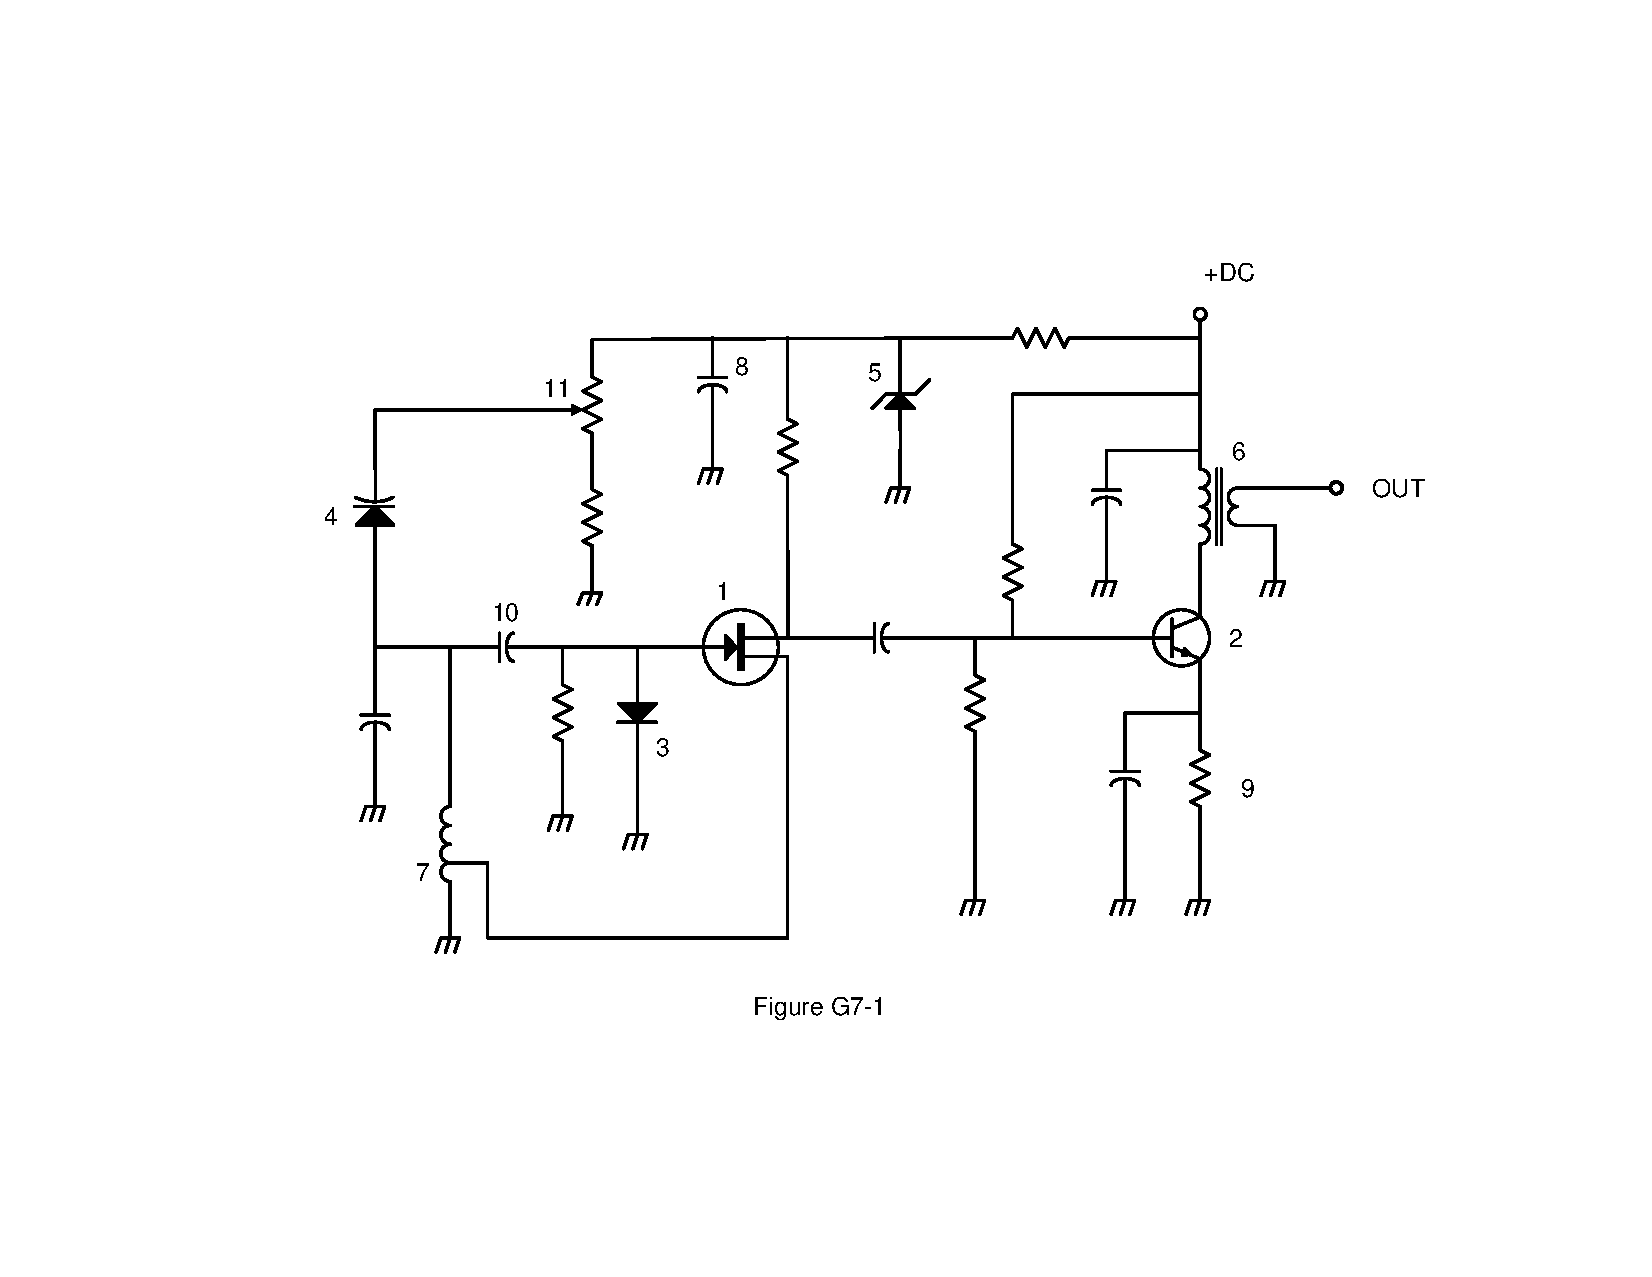
\includegraphics[width=\textwidth, keepaspectratio]{g7-1.pdf}
\end{center}

\section{G7B - Digital circuits; amplifiers and oscillators}

G7B01 (A) Complex digital circuitry can often be replaced by what type of integrated circuit?\\
A. Microcontroller\\

G7B02 (A) Which of the following is an advantage of using the binary system when processing digital signals?\\
A. Binary "ones" and "zeros" are easy to represent with an "on" or "off" state\\

G7B03 (B) Which of the following describes the function of a two input AND gate?\\
B. Output is high only when both inputs are high\\

G7B04 (C)  Which of the following describes the function of a two input NOR gate?\\
C. Output is low when either or both inputs are high\\

G7B05 (C) How many states does a 3-bit binary counter have?\\
C. 8\\

G7B06 (A) What is a shift register?\\
A. A clocked array of circuits that passes data in steps along the array\\

G7B07 (D) What are the basic components of virtually all sine wave oscillators?\\
D. A filter and an amplifier operating in a feedback loop \\

G7B08 (B) How is the efficiency of an RF power amplifier determined?\\
B. Divide the RF output power by the DC input power\\

G7B09 (C) What determines the frequency of an LC oscillator?\\
C. The inductance and capacitance in the tank circuit\\

G7B10 (D) Which of the following is a characteristic of a Class A amplifier?\\
D. Low distortion\\

G7B11 (B) For which of the following modes is a Class C power stage appropriate for amplifying a modulated signal?\\
B. CW\\

G7B12 (D) Which of these classes of amplifiers has the highest efficiency?\\
D. Class C\\

G7B13 (B) What is the reason for neutralizing the final amplifier stage of a transmitter?\\
B. To eliminate self-oscillations\\

G7B14 (B) Which of the following describes a linear amplifier?\\
B. An amplifier in which the output preserves the input waveform\\

\section{G7C - Receivers and transmitters; filters, oscillators}

G7C01 (B) Which of the following is used to process signals from the balanced modulator and send them to the mixer in a single-sideband phone transmitter?\\
B. Filter \\

G7C02 (D) Which circuit is used to combine signals from the carrier oscillator and speech amplifier and send the result to the filter in a typical single-sideband phone transmitter?\\
D. Balanced modulator\\

G7C03 (C) What circuit is used to process signals from the RF amplifier and local oscillator and send the result to the IF filter in a superheterodyne receiver?\\
C. Mixer\\

G7C04 (D) What circuit is used to combine signals from the IF amplifier and BFO and send the result to the AF amplifier in a single-sideband receiver?\\
D. Product detector\\

G7C05 (D) Which of the following is an advantage of a transceiver controlled by a direct digital synthesizer (DDS)?\\
D. Variable frequency with the stability of a crystal oscillator\\

G7C06 (B) What should be the impedance of a low-pass filter as compared to the impedance of the transmission line into which it is inserted? \\
B. About the same\\

G7C07 (C) What is the simplest combination of stages that implement a superheterodyne receiver?\\
C. HF oscillator, mixer, detector\\

G7C08 (D) What type of circuit is used in many FM receivers to convert signals coming from the IF amplifier to audio?\\
D. Discriminator\\

G7C09 (D) Which of the following is needed for a Digital Signal Processor IF filter?\\
A. An analog to digital converter\\
B. A digital to analog converter\\
C. A digital processor chip\\
D. All of the these choices are correct\\

G7C10 (B) How is Digital Signal Processor filtering accomplished?\\
B. By converting the signal from analog to digital and using digital processing\\

G7C11 (A) What is meant by the term "software defined radio" (SDR)?\\
A. A radio in which most major signal processing functions are performed by software\\

\chapter{Subelement G8 - Signals and Emissions: 2 Questions}
\section{G8A - Carriers and modulation: AM; FM; single and double sideband; modulation envelope; overmodulation}

G8A01 (D) What is the name of the process that changes the envelope of an RF wave to carry information?\\
D. Amplitude modulation\\

G8A02 (B) What is the name of the process that changes the phase angle of an RF wave to convey information?\\
B. Phase modulation\\

G8A03 (D) What is the name of the process which changes the frequency of an RF wave to convey information?\\
D. Frequency modulation\\

G8A04 (B) What emission is produced by a reactance modulator connected to an RF power amplifier?\\
B. Phase modulation\\

G8A05 (D) What type of modulation varies the instantaneous power level of the RF signal?\\
D. Amplitude modulation\\

G8A06 (C) What is one advantage of carrier suppression in a single-sideband phone transmission?\\
C. The available transmitter power can be used more effectively\\

G8A07 (A) Which of the following phone emissions uses the narrowest frequency bandwidth?\\
A. Single sideband\\

G8A08 (D) Which of the following is an effect of over-modulation?\\
D. Excessive bandwidth\\

G8A09 (B) What control is typically adjusted for proper ALC setting on an amateur single sideband transceiver?\\
B. Transmit audio or microphone gain\\

G8A10 (C) What is meant by flat-topping of a single-sideband phone transmission?\\
C. Signal distortion caused by excessive drive\\

G8A11 (A) What happens to the RF carrier signal when a modulating audio signal is applied to an FM transmitter?\\
A. The carrier frequency changes proportionally to the instantaneous amplitude of the modulating signal\\

G8A12 (A) What signal(s) would be found at the output of a properly adjusted balanced modulator?\\
A. Both upper and lower sidebands\\

\section{G8B - Frequency mixing; multiplication; HF data communications; bandwidths of various modes; deviation}

G8B01 (A) What receiver stage combines a 14.250 MHz input signal with a 13.795 MHz oscillator signal to produce a 455 kHz intermediate frequency (IF) signal?\\
A. Mixer\\

G8B02 (B) If a receiver mixes a 13.800 MHz VFO with a 14.255 MHz received signal to produce a 455 kHz intermediate frequency (IF) signal, what type of interference will a 13.345 MHz signal produce in the receiver?\\
B. Image response\\

G8B03 (A) What is another term for the mixing of two RF signals?\\
A. Heterodyning\\

G8B04 (D) What is the name of the stage in a VHF FM transmitter that generates a harmonic of a lower frequency signal to reach the desired operating frequency?\\
D. Multiplier\\

G8B05 (C) Why isn't frequency modulated (FM) phone used below 29.5 MHz?\\
C. The wide bandwidth is prohibited by FCC rules\\

G8B06 (D) What is the total bandwidth of an FM-phone transmission having a 5 kHz
deviation and a 3 kHz modulating frequency?\\
D. 16 kHz\\

G8B07 (B) What is the frequency deviation for a 12.21-MHz reactance-modulated oscillator in a 5-kHz deviation, 146.52-MHz FM-phone transmitter?\\
B. 416.7 Hz\\

G8B08 (B) Why is it important to know the duty cycle of the data mode you are using when transmitting?\\
B. Some modes have high duty cycles which could exceed the transmitter's average power rating.\\

G8B09 (D) Why is it good to match receiver bandwidth to the bandwidth of the operating mode?\\
D. It results in the best signal to noise ratio\\

G8B10 (A) What does the number 31 represent in PSK31?\\
A. The approximate transmitted symbol rate\\

G8B11 (C) How does forward error correction allow the receiver to correct errors in received data packets?\\
C. By transmitting redundant information with the data\\

G8B12 (B) What is the relationship between transmitted symbol rate and bandwidth?\\
B. Higher symbol rates require higher bandwidth\\

\chapter{Subelement G9 - Antennas and Feed Lines: 4 Questions}
\section{G9A - Antenna feed lines: characteristic impedance, and attenuation; SWR calculation, measurement and effects; matching networks}
 
G9A01 (A) Which of the following factors determine the characteristic impedance of a parallel conductor antenna feed line?\\
A. The distance between the centers of the conductors and the radius of the
conductors\\

G9A02 (B) What are the typical characteristic impedances of coaxial cables used for antenna feed lines at amateur stations?\\
B. 50 and 75 ohms\\

G9A03 (D) What is the characteristic impedance of flat ribbon TV type twinlead?\\
D. 300 ohms\\

G9A04 (C) What is the reason for the occurrence of reflected power at the point where a feed line connects to an antenna?\\
C. A difference between feed-line impedance and antenna feed-point impedance\\

G9A05 (B) How does the attenuation of coaxial cable change as the frequency of the signal it is carrying increases?\\
B. It increases\\

G9A06 (D) In what values are RF feed line losses usually expressed?\\
D. dB per 100 ft\\

G9A07 (D) What must be done to prevent standing waves on an antenna feed line?\\
D. The antenna feed-point impedance must be matched to the characteristic impedance of the feed line\\

G9A08 (B) If the SWR on an antenna feed line is 5 to 1, and a matching network at the transmitter end of the feed line is adjusted to 1 to 1 SWR, what is the resulting SWR on the feed line?\\
B. 5 to 1\\

G9A09 (A) What standing wave ratio will result from the connection of a 50-ohm feed line to a non-reactive load having a 200-ohm impedance?\\
A. 4:1\\

G9A10 (D) What standing wave ratio will result from the connection of a 50-ohm feed line to a non-reactive load having a 10-ohm impedance?\\
D. 5:1\\

G9A11 (B) What standing wave ratio will result from the connection of a 50-ohm feed line to a non-reactive load having a 50-ohm impedance?\\
B. 1:1\\

G9A12 (A) What would be the SWR if you feed a vertical antenna that has a 25-ohm feed-point impedance with 50-ohm coaxial cable?\\
A. 2:1\\

G9A13 (C) What would be the SWR if you feed an antenna that has a 300-ohm feed-point impedance with 50-ohm coaxial cable?\\
C. 6:1\\

\section{G9B - Basic antennas}


G9B01 (B) What is one disadvantage of a directly fed random-wire antenna?\\
B. You may experience RF burns when touching metal objects in your station \\

G9B02 (D) What is an advantage of downward sloping radials on a quarter wave ground-plane antenna?\\
D. They bring the feed-point impedance closer to 50 ohms\\

G9B03 (B) What happens to the feed-point impedance of a ground-plane antenna when its radials are changed from horizontal to downward-sloping?\\
B. It increases\\

G9B04 (A) What is the low angle azimuthal radiation pattern of an ideal half-wavelength dipole antenna installed 1/2 wavelength high and parallel to the Earth?\\
A. It is a figure-eight at right angles to the antenna\\

G9B05 (C) How does antenna height affect the horizontal (azimuthal) radiation pattern of a horizontal dipole HF antenna?\\
C. If the antenna is less than 1/2 wavelength high, the azimuthal pattern is almost omnidirectional\\

G9B06 (C) Where should the radial wires of a ground-mounted vertical antenna system be placed?\\
C. On the surface or buried a few inches below the ground\\

G9B07 (B) How does the feed-point impedance of a 1/2 wave dipole antenna change as the antenna is lowered from 1/4 wave above ground?\\
B. It steadily decreases\\

G9B08 (A) How does the feed-point impedance of a 1/2 wave dipole change as the feed-point location is moved from the center toward the ends?\\
A. It steadily increases\\

G9B09 (A) Which of the following is an advantage of a horizontally polarized as compared to vertically polarized HF antenna?\\
A. Lower ground reflection losses \\

G9B10 (D) What is the approximate length for a 1/2-wave dipole antenna cut for 14.250 MHz?\\
D. 32 feet\\

G9B11 (C) What is the approximate length for a 1/2-wave dipole antenna cut for 3.550 MHz?\\
C. 131 feet\\

G9B12 (A) What is the approximate length for a 1/4-wave vertical antenna cut for 28.5 MHz?\\
A. 8 feet\\

\section{G9C - Directional antennas}


G9C01 (A) Which of the following would increase the bandwidth of a Yagi antenna?\\
A. Larger diameter elements\\

G9C02 (B) What is the approximate length of the driven element of a Yagi antenna?\\
B. 1/2 wavelength\\

G9C03 (B) Which statement about a three-element, single-band Yagi antenna is true?\\
B. The director is normally the shortest parasitic element\\

G9C04 (A) Which statement about a three-element; single-band Yagi antenna is true?\\
A. The reflector is normally the longest parasitic element\\

G9C05 (A) How does increasing boom length and adding directors affect a Yagi antenna?\\
A. Gain increases\\

G9C06 (C) Which of the following is a reason why a Yagi antenna is often used for radio communications on the 20 meter band?\\
C. It helps reduce interference from other stations to the side or behind the antenna\\

G9C07 (C) What does "front-to-back ratio" mean in reference to a Yagi antenna?\\
C. The power radiated in the major radiation lobe compared to the power radiated in exactly the opposite direction\\

G9C08 (D) What is meant by the "main lobe" of a directive antenna?\\
D. The direction of maximum radiated field strength from the antenna\\

G9C09 (A) What is the approximate maximum theoretical forward gain of a three element, single-band Yagi antenna?\\
A. 9.7 dBi\\

G9C10 (D) Which of the following is a Yagi antenna design variable that could be adjusted to optimize forward gain, front-to-back ratio, or SWR bandwidth? \\
A. The physical length of the boom\\
B. The number of elements on the boom\\
C. The spacing of each element along the boom\\
D. All of these choices are correct\\

G9C11 (A) What is the purpose of a gamma match used with Yagi antennas?\\
A. To match the relatively low feed-point impedance to 50 ohms\\

G9C12 (A) Which of the following is an advantage of using a gamma match for impedance matching of a Yagi antenna to 50-ohm coax feed line?\\
A. It does not require that the elements be insulated from the boom\\

G9C13 (A) Approximately how long is each side of a quad antenna driven element?\\
A. 1/4 wavelength\\

G9C14 (B) How does the forward gain of a two-element quad antenna compare to the forward gain of a three-element Yagi antenna?\\
B. About the same\\

G9C15 (B) Approximately how long is each side of a quad antenna reflector element?\\
B. Slightly more than 1/4 wavelength\\

G9C16 (D) How does the gain of a two-element delta-loop beam compare to the gain of a two-element quad antenna?\\
D. About the same\\

G9C17 (B) Approximately how long is each leg of a symmetrical delta-loop antenna?\\
B. 1/3 wavelength\\

G9C18 (A) What happens when the feed point of a quad antenna is changed from the center of either horizontal wire to the center of either vertical wire?\\
A. The polarization of the radiated signal changes from horizontal to vertical\\

G9C19 (D) What configuration of the loops of a two-element quad antenna must be used for the antenna to operate as a beam antenna, assuming one of the elements is used as a reflector? \\
D. The reflector element must be approximately 5\% longer than the driven element\\

G9C20 (B) How does the gain of two 3-element horizontally polarized Yagi antennas spaced vertically 1/2 wavelength apart typically compare to the gain of a single 3-element Yagi?\\
B. Approximately 3 dB higher\\

\section{G9D - Specialized antennas}

G9D01 (D) What does the term "NVIS" mean as related to antennas?\\
D. Near Vertical Incidence Sky wave\\

G9D02 (B) Which of the following is an advantage of an NVIS antenna?\\
B. High vertical angle radiation for working stations within a radius of a few hundred kilometers\\

G9D03 (D) At what height above ground is an NVIS antenna typically installed?\\
D. Between 1/10 and 1/4 wavelength\\

G9D04 (A) What is the primary purpose of antenna traps?\\
A. To permit multiband operation\\

G9D05 (D) What is the advantage of vertical stacking of horizontally polarized Yagi antennas?\\
D. Narrows the main lobe in elevation\\

G9D06 (A) Which of the following is an advantage of a log periodic antenna?\\
A. Wide bandwidth\\

G9D07 (A) Which of the following describes a log periodic antenna?\\
A. Length and spacing of the elements increases logarithmically from one end of the boom to the other\\

G9D08 (B) Why is a Beverage antenna not used for transmitting?\\
B. It has high losses compared to other types of antennas\\

G9D09 (B) Which of the following is an application for a Beverage antenna?\\
B. Directional receiving for low HF bands\\

G9D10 (D) Which of the following describes a Beverage antenna?\\
D. A very long and low directional receiving antenna\\

G9D11 (D) Which of the following is a disadvantage of multiband antennas?\\
D. They have poor harmonic rejection\\

\chapter{Subelement G0 - Electrical and RF Safety: 2 Questions}
\section{G0A - RF safety principles, rules and guidelines; routine station evaluation}

G0A01 (A) What is one way that RF energy can affect human body tissue?\\
A. It heats body tissue\\

G0A02 (D) Which of the following properties is important in estimating whether an RF signal exceeds the maximum permissible exposure (MPE)?\\
A. Its duty cycle\\
B. Its frequency\\
C. Its power density\\
D. All of these choices are correct\\

G0A03 (D) [97.13(c)(1)] How can you determine that your station complies with FCC RF exposure regulations?\\
A. By calculation based on FCC OET Bulletin 65\\
B. By calculation based on computer modeling\\
C. By measurement of field strength using calibrated equipment\\
D. All of these choices are correct\\

G0A04 (D) What does "time averaging" mean in reference to RF radiation exposure?\\
D. The total RF exposure averaged over a certain time\\

G0A05 (A) What must you do if an evaluation of your station shows RF energy radiated from your station exceeds permissible limits?\\
A. Take action to prevent human exposure to the excessive RF fields\\

G0A07 (A) What effect does transmitter duty cycle have when evaluating RF exposure? \\
A. A lower transmitter duty cycle permits greater short-term exposure levels\\

G0A08 (C) Which of the following steps must an amateur operator take to ensure compliance with RF safety regulations when transmitter power exceeds levels specified in part 97.13?\\
C. Perform a routine RF exposure evaluation\\

G0A09 (B) What type of instrument can be used to accurately measure an RF field?\\
B. A calibrated field-strength meter with a calibrated antenna\\

G0A10 (D) What is one thing that can be done if evaluation shows that a neighbor might receive more than the allowable limit of RF exposure from the main lobe of a directional antenna?\\
D. Take precautions to ensure that the antenna cannot be pointed in their direction\\

G0A11 (C) What precaution should you take if you install an indoor transmitting antenna?\\
C. Make sure that MPE limits are not exceeded in occupied areas\\

G0A12 (B) What precaution should you take whenever you make adjustments or repairs to an antenna?\\
B. Turn off the transmitter and disconnect the feed line\\

G0A13 (D) What precaution should be taken when installing a ground-mounted antenna?\\
D. It should be installed so no one can be exposed to RF radiation in excess of maximum permissible limits\\

\section{G0B - Safety in the ham shack: electrical shock and treatment, safety grounding, fusing, interlocks, wiring, antenna and tower safety}


G0B01 (A) Which wire or wires in a four-conductor line cord should be attached to fuses or circuit breakers in a device operated from a 240-VAC single-phase source?\\
A. Only the hot wires \\

G0B02 (C) What is the minimum wire size that may be safely used for a circuit that draws up to 20 amperes of continuous current?\\
C. AWG number 12\\

G0B03 (D) Which size of fuse or circuit breaker would be appropriate to use with a circuit that uses AWG number 14 wiring? \\
D. 15 amperes\\

G0B04 (A) Which of the following is a primary reason for not placing a gasoline-fueled generator inside an occupied area?\\
A. Danger of carbon monoxide poisoning\\

G0B05 (B) Which of the following conditions will cause a Ground Fault Circuit Interrupter (GFCI) to disconnect the 120 or 240 Volt AC line power to a device?\\
B. Current flowing from one or more of the hot wires directly to ground\\

G0B06 (D)  Why must the metal enclosure of every item of station equipment be grounded?\\
D. It ensures that hazardous voltages cannot appear on the chassis\\

G0B07 (B) Which of the following should be observed for safety when climbing on a tower using a safety belt or harness?\\
B. Always attach the belt safety hook to the belt D-ring with the hook opening away from the tower\\

G0B08 (B) What should be done by any person preparing to climb a tower that supports electrically powered devices?\\
B. Make sure all circuits that supply power to the tower are locked out and tagged\\

G0B09 (D) Why should soldered joints not be used with the wires that connect the base of a tower to a system of ground rods?\\
D. A soldered joint will likely be destroyed by the heat of a lightning strike\\

G0B10 (A) Which of the following is a danger from lead-tin solder?\\
A. Lead can contaminate food if hands are not washed carefully after handling\\

G0B11 (D) Which of the following is good engineering practice for lightning protection grounds?\\
D. They must be bonded together with all other grounds\\

G0B12 (C) What is the purpose of a transmitter power supply interlock?\\
C. To ensure that dangerous voltages are removed if the cabinet is opened\\

G0B13 (A) What must you do when powering your house from an emergency generator?\\
A. Disconnect the incoming utility power feed\\

G0B14 (C) Which of the following is covered by the National Electrical Code?\\
C. Electrical safety inside the ham shack\\

G0B15 (A) Which of the following is true of an emergency generator installation?\\
A. The generator should be located in a well ventilated area \\

G0B16 (C) When might a lead acid storage battery give off explosive hydrogen gas?\\
C. When being charged\\
\end{document}